%%%%%%%%%%%%%%%%%%%%%%%%%%%%%%%%%%%%%%%%%
% Journal Article

%----------------------------------------------------------------------------------------
%	PACKAGES AND OTHER DOCUMENT CONFIGURATIONS
%----------------------------------------------------------------------------------------

\documentclass[twoside]{article}

%\pdfminorversion=4 % To be able to open the pdf afterwards

\usepackage{color} 

\newcommand{\labtitle}{Potash Mining Effluents Induce Moderate Effects on Histopathological and Endocrine Endpoints of Adult Zebrafish, \textit{Danio rerio}
}
\newcommand{\names}{}


\usepackage{lipsum} 
%\usepackage[british]{babel}
\usepackage{url}

% !TEX program = XeLaTeX
\usepackage{array} %for tables \setlength{\extrarowheight}{1.5pt}

\usepackage{amsmath}
\def\permille{\ensuremath{{}^\text{o}\mkern-5mu/\mkern-3mu_\text{oo}}}
\usepackage{braket} % Obvious
\usepackage{booktabs}
\setcounter{MaxMatrixCols}{20}
\newenvironment{Figure} % So the figures can be seen
  {\par\medskip\noindent\minipage{\linewidth}}
  {\endminipage\par\medskip}

\usepackage{helvet}
\usepackage{placeins}
%\usepackage[sc]{mathpazo} % Use the Palatino font
\usepackage[T1]{fontenc} % Use 8-bit encoding that has 256 glyphs
\linespread{1.5} % Line spacing - Palatino needs more space between lines
\usepackage{microtype} % Slightly tweak font spacing for aesthetics

\usepackage[hmarginratio=1:1,top=32mm,columnsep=20pt]{geometry} % Document margins
\usepackage{multicol} % Used for the two-column layout of the document
\usepackage[small,labelfont=bf,up,textfont=up]{caption} % Custom captions under/above floats in tables or figures
\usepackage{booktabs} % Horizontal rules in tables
\usepackage{float} % Required for tables and figures in the multi-column environment - they need to be placed in specific locations with the [H] (e.g. \begin{table}[H])
\usepackage{hyperref} % For hyperlinks in the PDF

\usepackage{textcase} % For lowercase

\usepackage{gensymb} % For Degree sign ° $^{\circ}$

\usepackage{lettrine} 
\usepackage{paralist} % Used for the compactitem environment which makes bullet points with less space between them
\usepackage[export]{adjustbox}

\usepackage{abstract} % Allows abstract customization
\renewcommand{\abstractnamefont}{\normalfont\bfseries} % Set the "Abstract" text to bold
\renewcommand{\abstracttextfont}{\normalfont\small} % Set the abstract itself to small italic text

\usepackage{titlesec} % Allows customization of titles
%\renewcommand\thesection{\Roman{section}} % Roman numerals for the sections
%\renewcommand\thesubsection{\Roman{subsection}} % Roman numerals for subsections
\titleformat{\section}[block]{\large\scshape\centering}{\thesection.}{1em}{} % Change the look of the section titles
\titleformat{\subsection}[block]{\large}{\thesubsection.}{1em}{} % Change the look of the section titles

\usepackage{fancyhdr} % Headers and footers
\pagestyle{fancy} % All pages have headers and footers
\fancyhead{} % Blank out the default header
\fancyfoot{} % Blank out the default footer
%\fancyhead[C]{Marine Ecology $\bullet$ BIO4408} % Custom header text
\fancyfoot[RO,LE]{\thepage} % Custom footer text

\usepackage{hyperref}
\usepackage{booktabs}
\usepackage{natbib}
\bibliographystyle{authordate1}
%----------------------------------------------------------------------------------------
%	TITLE SECTION
%----------------------------------------------------------------------------------------

\title{\vspace{-15mm}\fontsize{22pt}{11pt}\selectfont\textbf{\labtitle}} % Article title

\author{
\large
\textsc{\names}\\[2mm] Katja Irob, Marit Wagler, Nora Baberschke, Werner Kloas, Thomas Meinelt \\
%\normalsize \href{mailto:\emailone}{\emailone} \\ % Emails
\normalsize  Leibniz Institute of Freshwater Ecology, Berlin % Your institution
}

%\date{March 2017}



%----------------------------------------------------------------------------------------

\begin{document}

\maketitle % Insert title

\thispagestyle{fancy} % All pages have headers and footers

%----------------------------------------------------------------------------------------
%	ABSTRACT
%----------------------------------------------------------------------------------------
\begin{abstract}

\end{abstract}

\textbf{Keywords: secondary river salinisation, freshwater fish, ion imbalances, osmoregulatory stress, wastewater management}


%----------------------------------------------------------------------------------------
%	ARTICLE CONTENTS
%----------------------------------------------------------------------------------------

\begin{multicols}{2} % Two-column layout throughout the main article text
\section{Introduction}
\lettrine[nindent=0em,lines=2]{S}{}

econdary salinisation of rivers due to progressive human activity is a global problem, increasingly affecting countries all around the world \citep{Arle2013,Canedo2013,Silva2000,Williams2001}. Salinisation can be classified as either primary or secondary, depending on its origin. Primary salinisation is caused by natural processes, such as weathering of rocks, evaporation and precipitation, whereas secondary salinisation is due to anthropogenic actions \citep{Canedo2012}.\\
In Germany, a severe case of secondary salinisation is caused by the release of potash mining effluents into river systems.These effluents arise as a consequence of the the mining and processing of potash salts. They hold, beneath others, a vast portion of chloride (Cl$^-$),  magnesium (Mg$^{2+}$), potassium ( K$^+$) and sodium (Na$^+$) and are discharged either directly or indirectly into surface waters nearby.  \\
The affected River Werra is considered to be one of the most ecologically disturbed European freshwater ecosystems. Almost all biological metrics relevant for ecological status classification under EU-Water Framework Directive (EU-WFD) were adversely affected, causing the Werra to fall into their worst category, 'bad' \citep{Arle2013}.  \\

The river Werra has shown a large decline decline in diversity and abundance of local species, together with poor health as well as structural changes of biocoenosis  \citep{Arle2013,hubner2007}. Electrofishing data from 2010 to 2017 show, that in the River Werra, compared to a neighbouring undisturbed river, fish density was substantially lower and disease characteristics are significantly higher \citep{Laves2017}.  Furthermore, subadult or adult individuals are more frequently present compared to intermediate age cohorts, which are often completely absent (Schwevers et al., 2005). 
 %%citation  !!!! %%%%%%%%
\\
Regardless, threshold values only exist for Cl$^-$, Mg$^{2+}$ and K$^+$ concentrations, as well as total hardness, without scientifically validated reference values \citep{hubner2006}.\\ \\

Despite efficient mechanisms evolved to maintain the hydromineral homeostasis, high concentrations and imbalances of essential ions can lead to osmotic stress and eventually impair physiological functions of freshwater organisms \citep{goodfellow2000,mount1997}. Disturbances of ion homeostasis include various acute effects, like the release of stress hormones, mobilisation of energy resources and alterations of the diffusing capacity in gills due to changes in gill structure \citep{Mcdonald1997,bonga1997}.\\ 

The hormone cortisol has many different functions, the two major roles are regulation of the hydromineral balance and of energy metabolism, e.g. mobilisation of energy-rich substrates under stressful conditions and high energetic demand. It also influences growth rate as well as reproductive and immune functions \citep{bonga1997,pickering1981}. 
Together with the growth hormone (GH), cortisol controls the hydromineral balance. Jointly they control the acclimation response of teleost gill in governing cell turnover in osmoregulatory epithelia \citep{Mccormick2001,Evans2008}. GH induces the differentiation of seawater chloride cell during seawater acclimatisation, whereas prolactin (PRO) promotes cell proliferation during freshwater acclimatisation and has an inhibitory effect on the formation of seawater chloride cells \citep{Sakamoto2006}. \\ \\
The gonadotropins FSH (follicle-stimulating hormone) and LH (luteinising hormone) are the most important mediators of vertebrate reproduction and have both been identified to play a role in ovarian growth and gonadal maturation \citep{So2005}. 
Effects of stress on these hormones, described by several studies, include decrease in gamete quality, fertilisation success, and hatchability \citep{Schlenk2001,Schreck2001}. \\ \\
Many studies address the effects of high NaCl concentrations on freshwater fish ranging from adaptation to increased mortality \citep{shahriari2013}, however, knowledge about physiological effects of single ions and ion imbalances remain scarce. \citep{hubner2007,Canedo2012,goodfellow2000}. \citeauthor{mount1997} (1997) detected effects of single ions, such as potassium (K$^+$), as one of the major ions influencing toxicity. \\
Increased K$^+$ concentrations can affect various membrane functions and can severely impact vital diffusion processes (Wegner, 2016). Increases in serum K$^+$ ions related to renal osmoregulatory failure after copper exposure in marine sheepshead were considered to be life-threatening \cite{cardeilhac1979}. 
Mg${^2+}$ influences physical osmotic and membrane diffusion processes in aquatic organisms. Fluctuations of metabolically relevant ions, such as Mg${^2+}$ and K$^+$, can cause stress and can, in the worst case, cause a massive decline in those organisms who are unable to re-establish homeostasis \citep{wegner2016}. \\


Furthermore, the acute toxicity of different potash salt concentrations on juvenile zebra fish was confirmed by \cite{meinelt2008}. A significant percentage of larvae exposed to different potash concentrations ranging from $2 - 8\permille$ did not survive and most survivors were characterised by deformations. Even low concentrations can be toxic and lead to mortality \citep{meinelt2008}. \\ \\ 

The aim of this study was to investigate the effects of high concentrations and imbalances of major ions on the model organism and freshwater fish; \textit{Danio rerio}. High concentrations of ions representing the current and future threshold values were evaluated and ion imbalances were investigated in order to assess the potential toxicity of K$^+$ and Mg${^2+}$. It was hypothesised, that performance of zebrafish would be especially impaired by the exposure representing current thresholds  as well as high K$^+$ concentrations. 

%%%%%%%%%%%%%%%%%%%%%%
%%%%%%%%%%%%%%%%%%%%%%%
\section{Materials \& methods}
Adult zebrafish (60 males and 60 females) were obtained from a breeding stock of the Leibniz-Institute of Freshwater Ecology and Inland Fisheries (IGB), Berlin, Germany (females: length = 40.23 $\pm$ 1.89 mm, weight = 769.15 $\pm$ 66.96 mg; males: length = 37.03 $\pm$ 1.33, weight = 478.59 $\pm$ 35.94 mg). \\
Two males and two females were randomly kept together under flow-through conditions (5-fold flow-through/day, 1.4 L/h) in 7 L breeding tanks. The light:dark cycle was 12:12 h, temperature was kept at 25.85 $\pm$ 0.36 $^{\circ}$C (monitored daily) and fish were fed thrice a day ad libitum using freshly hatched Artemia salina nauplii and commercial flake food (Tetramin, Tetra, Germany). After a two-week acclimatisation period, fish were exposed to five test ion solutions (salts obtained from S3 Chemicals, Germany) for six weeks. The control group (ctrl) was held in processed tap water (Tab.:\ref{tab:testw}).\\
Ion concentrations in HT match legal threshold values until 2020 in Germany and LT depicts the anticipated concentration from 2021. 
Furthermore, ion solutions with a high Mg$^{2+ }$ and K$^+$ content (KMg),  high Mg$^{2+ }$ (Mg) and high K$^+$ (K) were evaluated. 
\\ A multichannel peristaltic pump, constantly adding the concentrated ion solutions, was used and calibrated daily.  The ion concentrations were verified weekly by ion chromatography (IC, Shimadzu, Japan) and inductively coupled plasma optical emission spectrometer (ICP-OES, Thermo Fisher Scientific, USA) and remained within 20\% deviation. To ensure that test conditions were kept according to OECD guidelines (Test No. 229), nitrite (NO$_2$$^-$= 0.026 $\pm$ 0.009 mg/L) and ammonium (NH$_4$$^+$= 0.051 $\pm$ 0.009 mg/L), pH (pH 7.94 $\pm$ 0.14), oxygen content (.52 $\pm$ 0.35 mg/L), temperature, conductivity and light intensity (536 $\pm$ 107 lux ) were controlled on a weekly basis. 

\begin{table}[H]
\centering
\caption{Concentration of single ions as well as mean conductivity $\pm$ SD measured in respective group.}
\label{tab:testw}
\adjustbox{width=1.0\columnwidth}{
\begin{tabular}{@{}lllllllll@{}}
\toprule
         & \begin{tabular}[c]{@{}l@{}}Ca$^{2+}$ \\ {[}mg/L{]}\end{tabular} & \begin{tabular}[c]{@{}l@{}}K$^+$\\ {[}mg/L{]}\end{tabular} & \begin{tabular}[c]{@{}l@{}}Mg$^{2+}$\\ {[}mg/L{]}\end{tabular} & \begin{tabular}[c]{@{}l@{}}Na$^+$\\ {[}mg/L{]}\end{tabular} & \begin{tabular}[c]{@{}l@{}}Cl$^-$\\ {[}mg/L{]}\end{tabular} & \begin{tabular}[c]{@{}l@{}}SO$_4^{2-}$\\ {[}mg/L{]}\end{tabular} & \begin{tabular}[c]{@{}l@{}}Mean\\ Conductivity\\ {[}ms/cm{]}\end{tabular} & \begin{tabular}[c]{@{}l@{}}sd\\ Conductivity\end{tabular} \\ \midrule
Ctrl & 76.47                                                      & 4.55                                                   & 8.75                                                      & 92.00                                                    & 57.69                                                    & 157.71                                                     & 0.84                                                                      & 0.01                                                      \\
HT & 176.60                                                     & 210.88                                                 & 330.50                                                    & 1137.50                                                  & 2307.50                                                  & 632.92                                                     & 7.98                                                                      & 0.54                                                      \\
LT   & 132.99                                                     & 144.65                                                 & 237.29                                                    & 752.50                                                   & 1651.10                                                  & 351.02                                                     & 5.29                                                                      & 0.46                                                      \\
KMg      & 122.47                                                     & 184.58                                                 & 361.13                                                    & 159.63                                                   & 53.48                                                    & 1813.43                                                    & 3.10                                                                      & 0.20                                                      \\
Mg       & 121.77                                                     & 13.05                                                  & 310.73                                                    & 159.13                                                   & 51.76                                                    & 1137.61                                                    & 2.50                                                                      & 0.38                                                      \\
K        & 93.62                                                      & 195.32                                                 & 11.25                                                     & 115.50                                                   & 58.9                                                     & 874.40                                                     & 1.38                                                                      & 0.05                                                      \\ \bottomrule
\end{tabular}}
\end{table}

\subsection{Animal Sampling}

Fish were starved 24 h prior to the end of the exposure period. At the sampling day, fish were sedated and euthanised in ice-water, total and standard length as well as weight were assessed. Four males and four females per exposure group were used for cortisol measurement. Gills and gonads were removed for histopathological analyses. The pituitary for mRNA expression analyses was snap frozen and stored at -80 $^{\circ}$C until RNA extraction was performed.


\subsection{Cortisol Extraction and ELISA}

Cortistol extraction was carried out after a modified version by \cite{canavello2011}. \\
Prior to the ELISA assay, samples  were stored at -20$^{\circ}$C and were then reconstituted in 500 ${\mu}$L phosphate-buffered saline (PBS). Quantification of cortisol concentrations were performed following the instructions of a human salivary cortisol assay kit (IBL International GmbH, Germany). \\
Absorbance was measured in a plate reader at 450 nm (Tecan infinite M200, Agilent, USA) and concentrations determined using a cubic spline fitting method, which were reported as relative circulating cortisol concentrations (ng/g body weight).  

\subsection{Relative Condition Factor}
The relative condition factor (RCF) was determined using body weight (W) in g and lenght (L) in mm:  
\begin{equation}
RCF = \frac{W}{(a\cdot L^{b})}
\end{equation}

The parameters \textit{a} and \textit{b} were estimated using data from the control group by log \textit{W} = log \textit{a} + \textit{b} log \textit{L}. Parameter \textit{a} denotes the regression intercept and \textit{b} the regression slope. \\ 
This condition factor compensates for changes in form or condition with increase in length. Here, it measures the deviation of an individual from the average weight for length in the control group. \\
RCF was determined prior to the exposure and at the end of the exposure. Males and females were analysed separately. 


\subsection{Histology}
Gonads and gills were removed, weight recorded and subsequently placed in embedding cassettes and fixed in Bouin's solution (Roth, Germany). The samples were dehydrated in a Shandon Excelsior$^{EM}$ ES tissue processor and afterwards manually embedded in paraffin blocks. 
Sections were carried out using a rotary microtome (Leica, Germany), where gills were cut at 3 $\mu$m and gonads at 4 $\mu$m.  Finally, all object slides were stained using hematoxylin and eosin (Roth, Germany).

\subsubsection{Gill Histology Evaluation}
Gill morphological alterations were evaluated under a light-microscope (Olympus, Japan) at x40 magnification and classified into different diagnostic criteria. Proliferation/hyperplasia  on primary and secondary filaments, fusion of filaments as well as lifting of epithelia/epithelia rupture/oedema. 
The degrees corresponded to the magnitude of the respective alteration (healthy = one to two layers of cells in interlamellar region, 'moderately' = three to five, 'severely' >= five layers). Three primary filaments each with 20 secondary filaments were analysed and means compared.

\subsubsection{Gonad Histology Evaluation}
Gonadal staging of zebrafish ovaries and testes was performed by processing digital microscopic photographs in an image analysis package (AnalySIS; Soft Imaging System, Germany). Sections were examined through a light-microscope (Leica, Germany) and photos were taken using an Olympus XC50 camera. 

\subsubsection{Ovaries}
One field of the average size of 2.25 mm$^2$ was outlined at x4 magnification at the centre of a section.
Gonadal stages were categorised in primary/perinucleolar oocytes (PO), cortical alveolar oocytes (CO), early vitellogenic oocytes (EV) and late vitellogenic oocytes (LV), which included mature/spawning oocytes \citep{Johnson2009}. \\
All follicles were quantified and the relative number and size of oocytes in each stage determined. Size was determined by area measurement.



\subsubsection{Testes}
For the analysis of testicular maturation, three random fields of view (0.2 mm$^2$) were analysed at x40 magnification. Spermatogenic cysts were classified into spermatids (ST), spermatocytes (SC) and spermatogonia (SG) \citep{Johnson2009}.


\subsection{mRNA Expression}

\subsubsection{RNA Extraction and Reverse Transcription}

Extraction of pituitary mRNA was carried out using an RNeasy-plus kit (Quiagen) according to the manufacturer's instructions. RNA concentrations were determined using RiboGreen following the manufacturer's protocol (Invitrogen). 
Extinction was measured using a plate reader (Tecan infinite M200, Agilent). \\

A subset of RNA samples was used to determine RNA integrity numbers (RIN, Agilent 2100 bioanalyser, Agilent Technologies), ranging between 7.1 and 9.1. Reverse transcription of RNA was conducted using a thermocycler (Biometra, G{\"o}ttingen).
%%hier genauer spezifizieren was gemacht wurde, aber unsicher welche infos genau wichtig sind 


\subsubsection{Quantitative Real Time PCR}
 RT-qPCR Primer sequences for \textit{lh} and \textit{gh} were obtained from 
\citep{lin2009} and \textit{fsh} from \citep{Xiaoying2014}. 
Prolactin primers were designed using Primer3 (Tab. \ref{tab:pcr}).\\
All PCR products were sequenced (SEQULAB, G{\"o}ttingen) and analysed with the database homology search tool BLAST (NCBI, USA) and multiple alignment sequence comparison. Sequence information was submitted to NCBI. Efficiency measurement for each primer was conducted in triplicates by using pooled mRNA in a dilution series. RT-qPCR was performed in duplicates in a Mx3005P qPCR Cycler (Stratagene), using hot start Taq-polymerase (Platinum, Invitrogen) and SYBR Green (Invitrogen) in a 20 ${\mu}$l reaction volume containing  2 ${\mu}$l cDNA. The comparative method (Δ Δ Ct method), melting curve analysis... %%insert
mRNA expressions were normalized relative to the housekeeping gene L8... %%insert PCR data 



%%%%muss noch in ne bessere Größe gepackt werden, VIEL zu klein 

\begin{table}[H]
\centering
\caption{Overview of qPCR conditions.}
\label{tab:pcr}
\adjustbox{width=1.0\columnwidth}{
\begin{tabular}{   l  l  l  l  l  l  l  }
\hline
	\textbf{Target gene} &\textbf{Primer} & \textbf{Sequence} & \textbf{T} & \textbf{Primer} &\textbf{MgCl$_2$} & \textbf{Product}  \\
    gene & &  & \textbf{[$^{\circ}$C]} & \textbf{[nM]} & \textbf{[nM]} & \textbf{size [bp]}  \\ \hline
	 \textbf{fsh*} & \textbf{forward} & TGAGCGCAGAATCAGAATG & 62 & 188 & 2 & 105  \\ 
     & \textbf{reverse} & AGGCTGTGGTGTCGATTGT & & & & \\
    \textbf{lh **} & \textbf{forward} & GCAGAGACACTTACAACAGCC & 64 & 375 & 2  & 145\\
     & \textbf{reverse} & AAAACCAAGCTCTGAGCAGCC & & & & \\
      \textbf{gh **} & \textbf{forward} &  CGAGACGCCGACGGGAAAAG & 64 & 375 & 2  & 271\\
     & \textbf{reverse} &  CGGCAGGGAGTCGTTGTCATC & & & & \\
      \textbf{pro ***} & \textbf{forward} & CAACCTGTCCACTCTCCCGT & 64 & 188 &2 & 210 \\
     & \textbf{reverse} & GCATTCACACCGAGAGCAGC & & & & \\
   \hline
\end{tabular}}
\end{table}
\FloatBarrier


\subsection{Statistics}
All data were analysed in the statistical software RStudio (RStudio, Inc., USA). ANOVAs and Post-Hoc Tukey's HSD tests were conducted for normally distributed data. For data deviating from a normal distribution, the non-parametric Kruskal-Wallis-Rank-Test and Dunn's multiple comparison test were carried out. To enhance the statistical power, different post-hoc p-value adjustment methods were applied (Holm, Chi-Square).  P-values lower than 0.05 are referred to as 'significant' and values below 0.001 as 'highly significant'. 

\section{Results}  

\subsection{Whole-body Cortisol}
In relation to ctrl, whole body cortisol was significantly higher in HT and K. Both were also significantly higher than KMg. 



\begin{figure}[H]
 \centering
 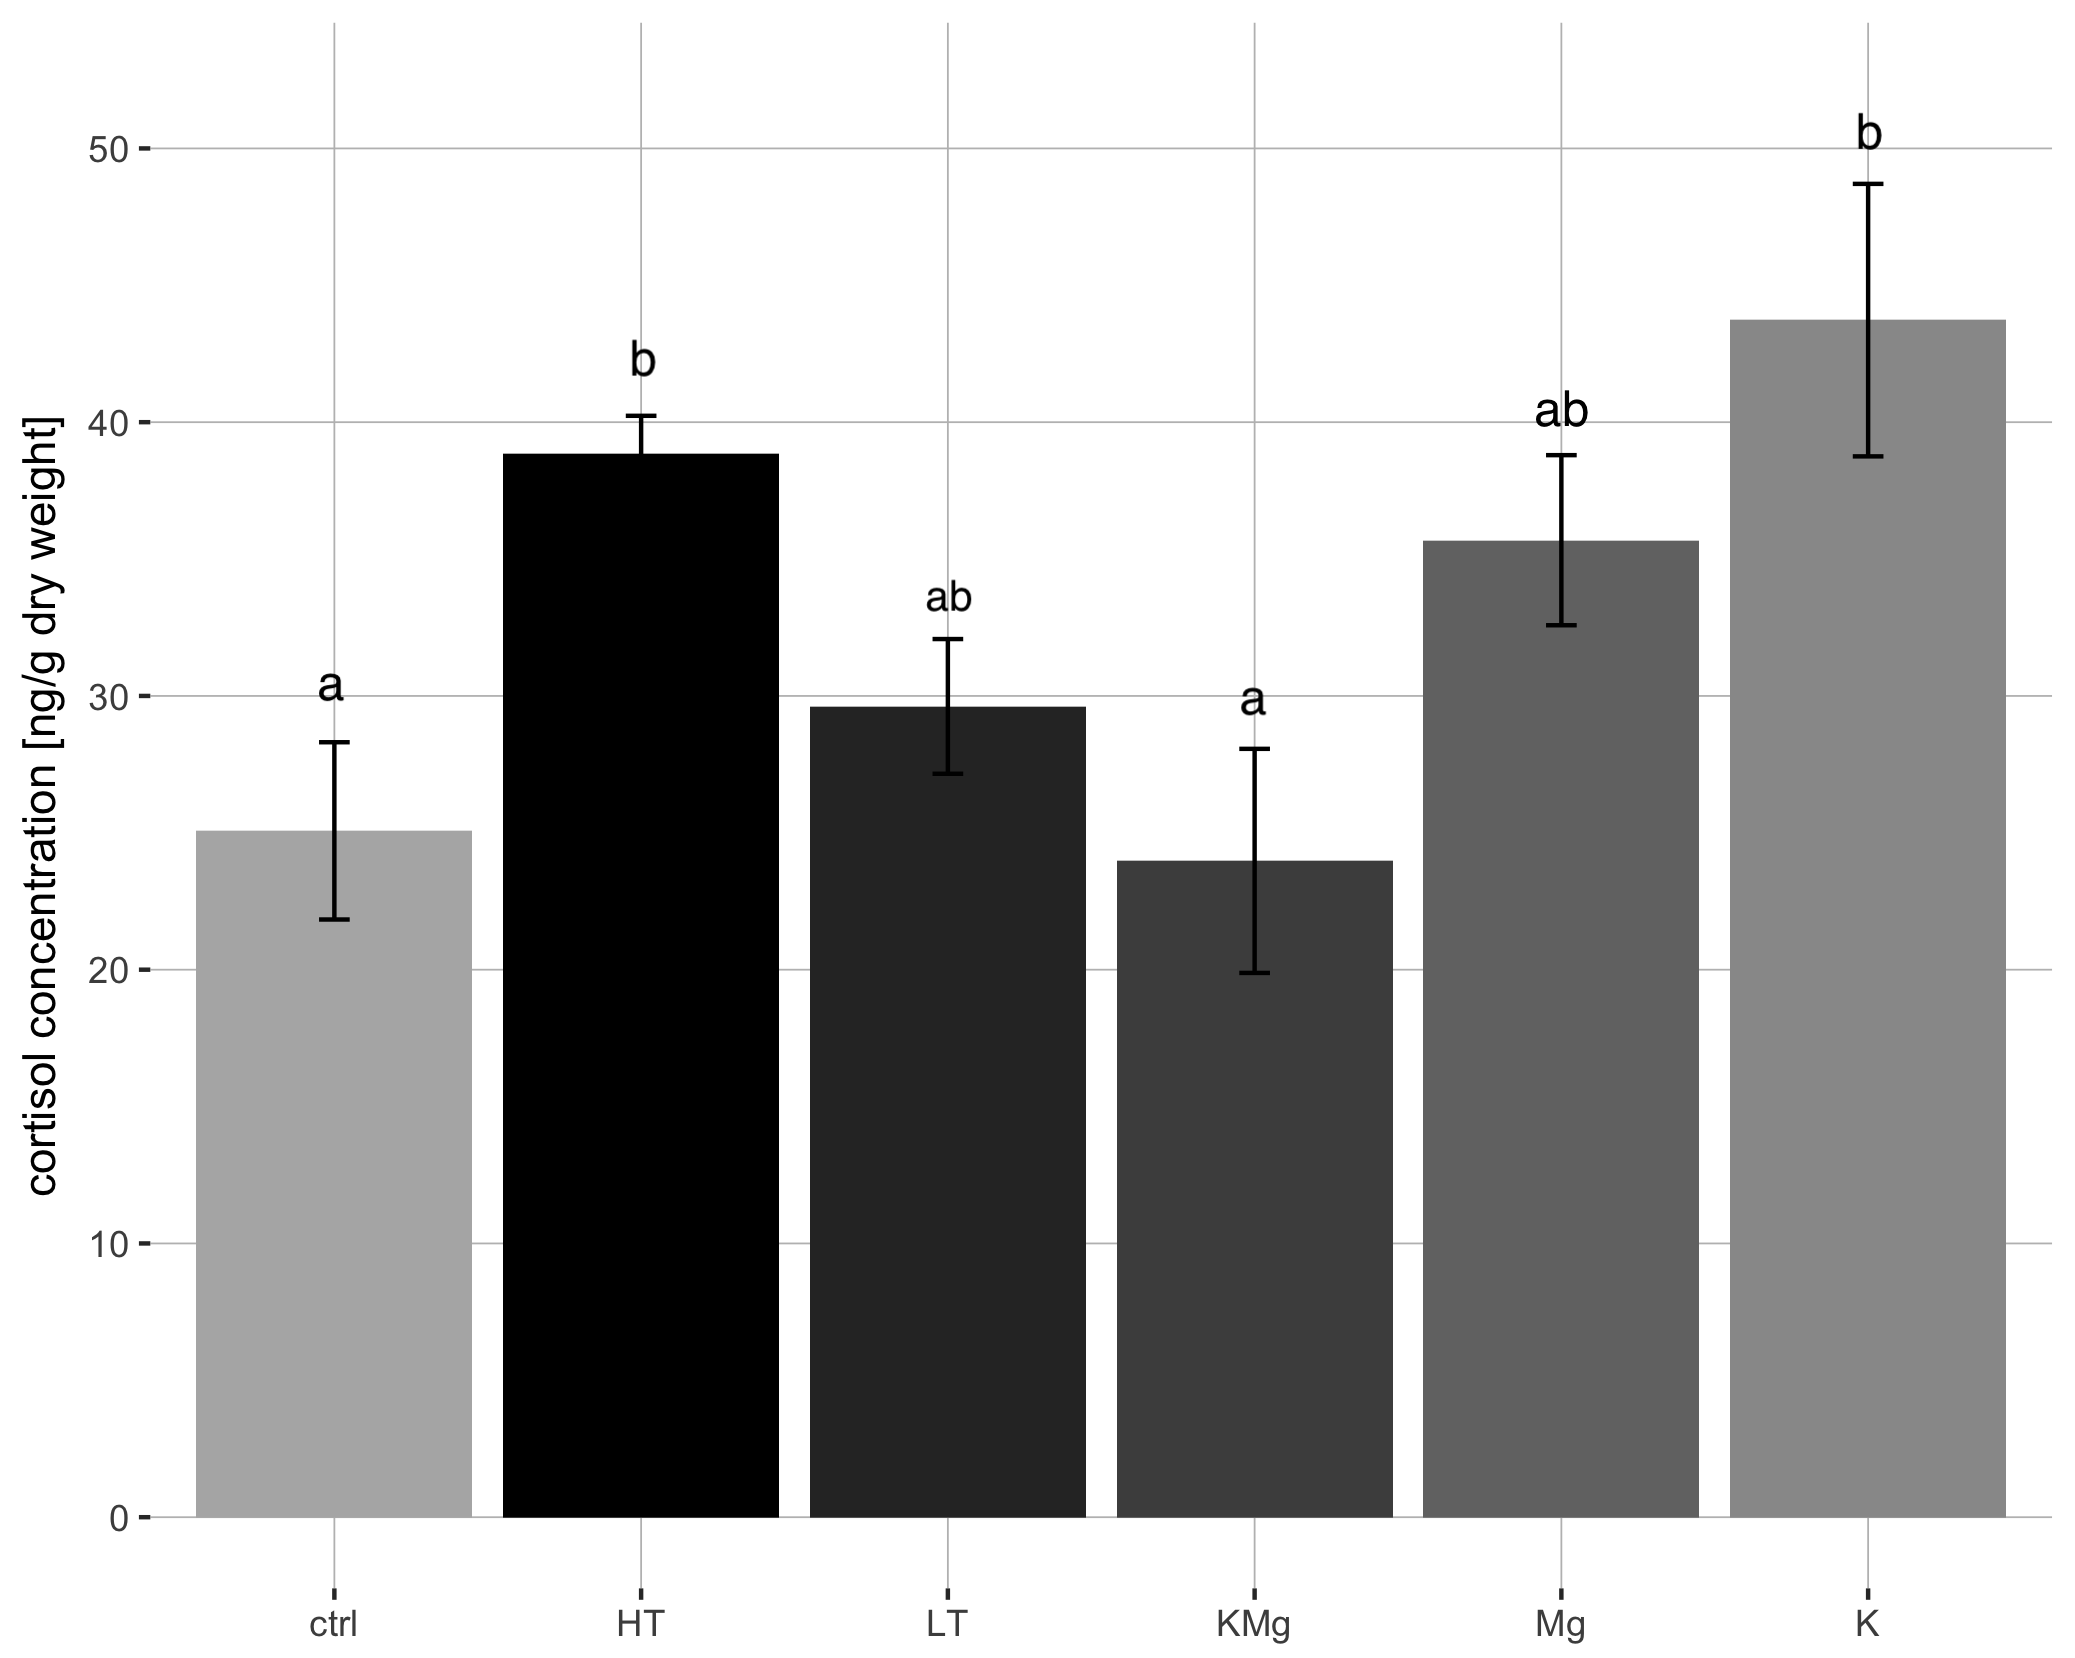
\includegraphics[scale=.1]{cortisol2205.png}
\captionof{figure}{Mean whole-body cortisol concentration [ng/g dry weight] $\pm$ SE for all exposure groups. $^{a,b}$ indicate significant differences by one-way ANOVA and Tukey test (p < 0.05, \textit{N = 6}).}
 \label{fig:cort}
\end{figure}
\FloatBarrier

\subsection{Relative Condition Factor}
At the beginning of the exposure, no significant difference for the weight-length relationship between the exposure groups and ctrl was found. \\ %fig 
More differences were found at the end of the exposure in both, within a group and between groups. However, no significant differences in RCFs were found for females. In males, RCF was significantly higher in HT compared to ctrl. 


\subsection{Gills}
The result of comparisons for each alteration of the gills between groups revealed a consistent significant difference between the exposure groups and ctrl, Fig.:\ref{fig:gills}. \\

All exposure groups were significantly different in their number of lamellar deformations from ctrl, but there were no differences between these. Besides, no significant difference between the sexes could be found. 
Exposed groups were characterised by hyperplasia between secondary lamellae and distal region of the secondary filament, which occasionally led to fusion of adjacent secondary lamellae. In addition to lifting of epithelia, oedema and rupture of epithelium were noted.
\\
Differences were highly significant for all three degrees of severity for hyperplasic filaments, compared to ctrl. \\

A higher mean number of minimally, moderately and severely lifted filaments was found for all exposure groups compared to ctrl. Additionally, Mg and K were significantly different in their mean number of minimally lifted filaments. 
Fusion of secondary lamellae was not a very common symptom, merely the amount of fused filaments between ctrl and HT was significantly different, Fig.:\ref{fig:gills}. No statistical difference between the exposure groups was found.



\end{multicols}

\begin{figure}[H]
 \centering
 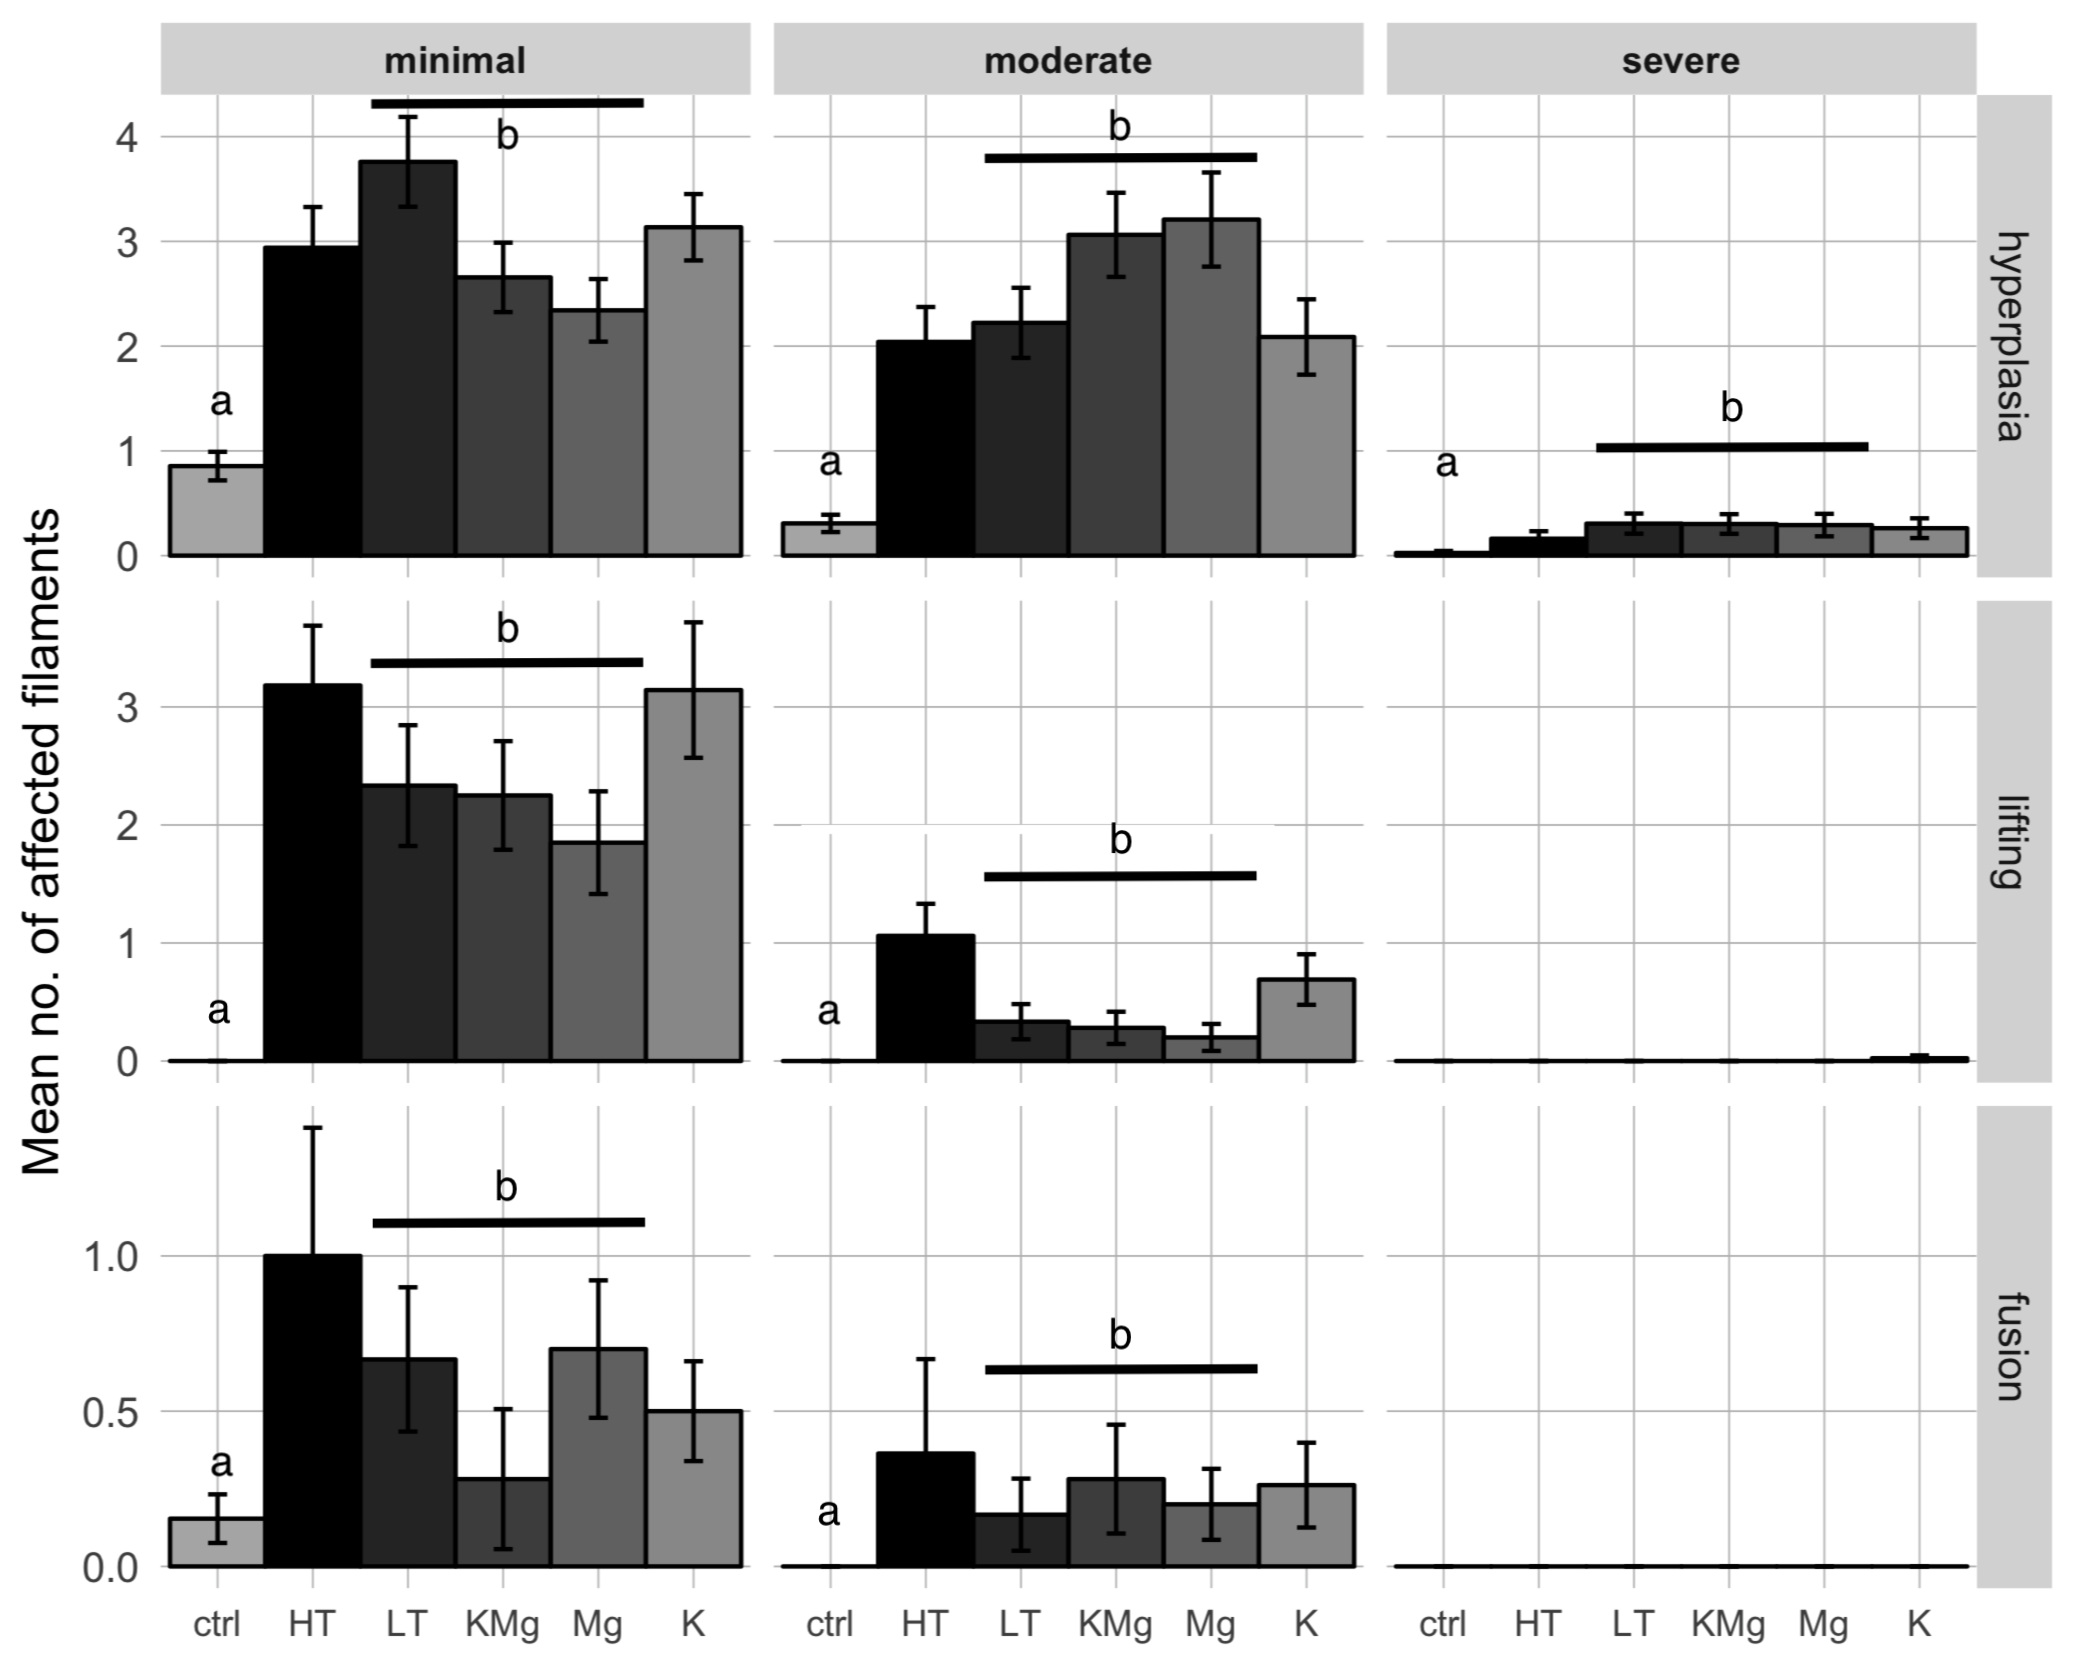
\includegraphics[scale=.185]{ggbarplot_gills2305.png}
\captionof{figure}{Mean number of affected filaments $\pm$ SE per primary gill filament for every diagnosis and exposure group. $^{a,b,c,d}$ indicate significant differences by Kruskal-Wallis and Dunn's test (p < 0.05). Sample size ranging from \textit{N = 8} to \textit{N = 10} per group.}
 \label{fig:gills}
\end{figure}
\FloatBarrier

\begin{multicols}{2}

\subsection{Gonads}
\subsubsection{Gonadosomatic Index (GSI)}
The GSI of females was significantly higher in LT than in ctrl. No differences were found for males. 

\begin{table}[H]
\centering
\caption{Mean GSI values for both sexes in all groups $\pm$ SD}
\label{tab:GSI}
\adjustbox{width=0.9\columnwidth}{
\begin{tabular}{@{}llll@{}}
\toprule
\textbf{Exposure Group} & \textbf{Sex} & \textbf{Mean GSI {[}\%{]}} & \textbf{SD} \\ \midrule
ctrl            & m            & 0.99                        & 0.12         \\
                   & f            & 10.39 \textbf{*}                    & 1.51        \\
HT           & m            & 0.99                        & 0.11         \\
                   & f            & 12.01                      & 1.77        \\
LT              & m            & 0.98                        & 0.12         \\
                   & f            & 15.63 \textbf{*}                     & 2.15        \\
KMg                & m            & 0.96                        & 0.17         \\
                   & f            & 10.91                      & 1.03        \\
Mg                 & m            & 1.12                       & 0.09         \\
                   & f            & 12.64                      & 2.05        \\
K                  & m            & 1.15                       & 0.11         \\
                   & f            & 11.80                      & 0.99         \\ \bottomrule
\end{tabular}}
\end{table}
\FloatBarrier 


\subsubsection{Ovaries}
Oocytes of each stage were present with some variation in the relative presence for each treatment, Fig.:\ref{fig:ovo}. 
Generally, there is a significant variation in size for all groups. \\
In the primary growth phase, perinucleolar oocytes (po) were significantly bigger in KMg compared to ctrl, as well as to Mg. 
Cortical aveoli oocytes (co) from KMg were highly significantly smaller than in ctrl and significantly smaller than in HT, LT, Mg and K. \\
In the early vitellogenic phase (ev), KMg was highly significantly smaller compared to ctrl.   Group size also differed highly significantly between KMg and HT, with KMg being significantly smaller. \\
The size of late vitellogenic oocytes (lv) in K were highly significantly bigger than in HT and KMg.  LT was also significantly bigger in size than KMg.


\begin{figure}[H]
 \centering
 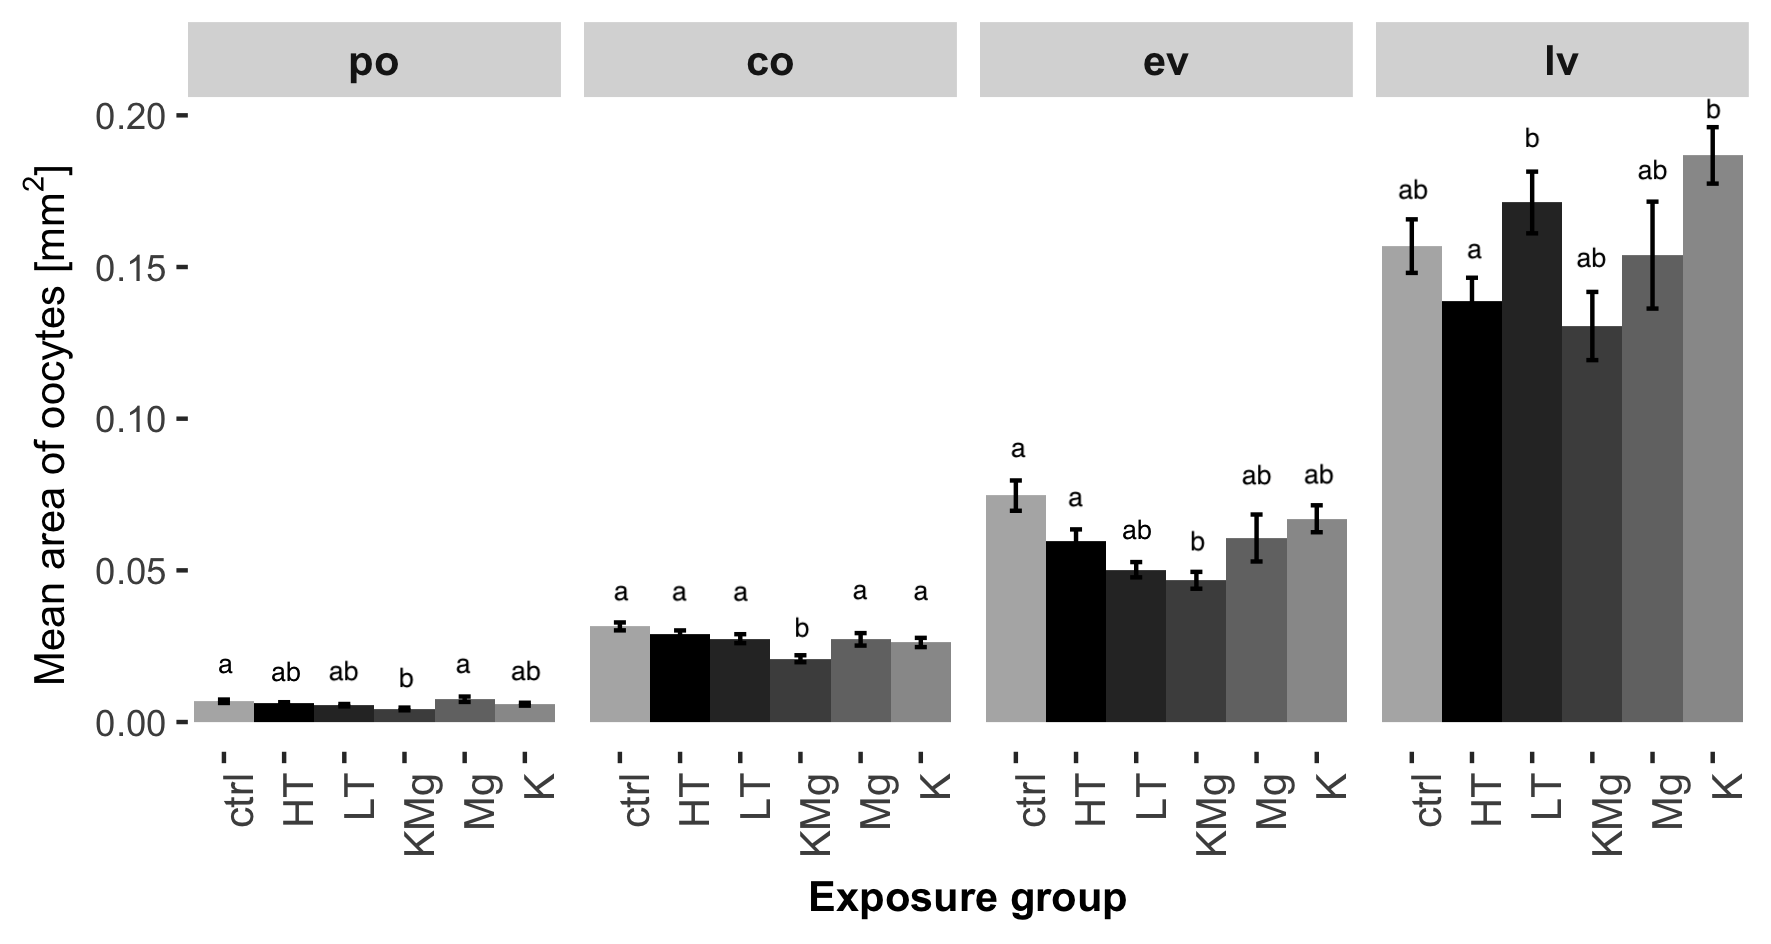
\includegraphics[scale=.117]{ggbarlot_ovaarea_2.png}
\captionof{figure}{Mean area size of developing oocytes $\pm$ SE for all groups in each stage. $^{a,b}$ indicate significant differences by one-way ANOVA and Tukey test (p < 0.05, \textit{N = 10}).}
 \label{fig:ovo}
\end{figure}
\FloatBarrier

Regarding the quantitative distribution of oocytes, there are no significant differences in the pre-vitellogenic stages po and co.\\  A significantly different distribution of ev oocytes was found between ctrl and KMg, with KMg having highly significantly more than ctrl. KMg also had highly significantly more than HT. \\
For lv, a significant difference between ctrl and LT was found, with LT lv oocytes being more abundant than ctrl. 


\begin{figure}[H]
 \centering
 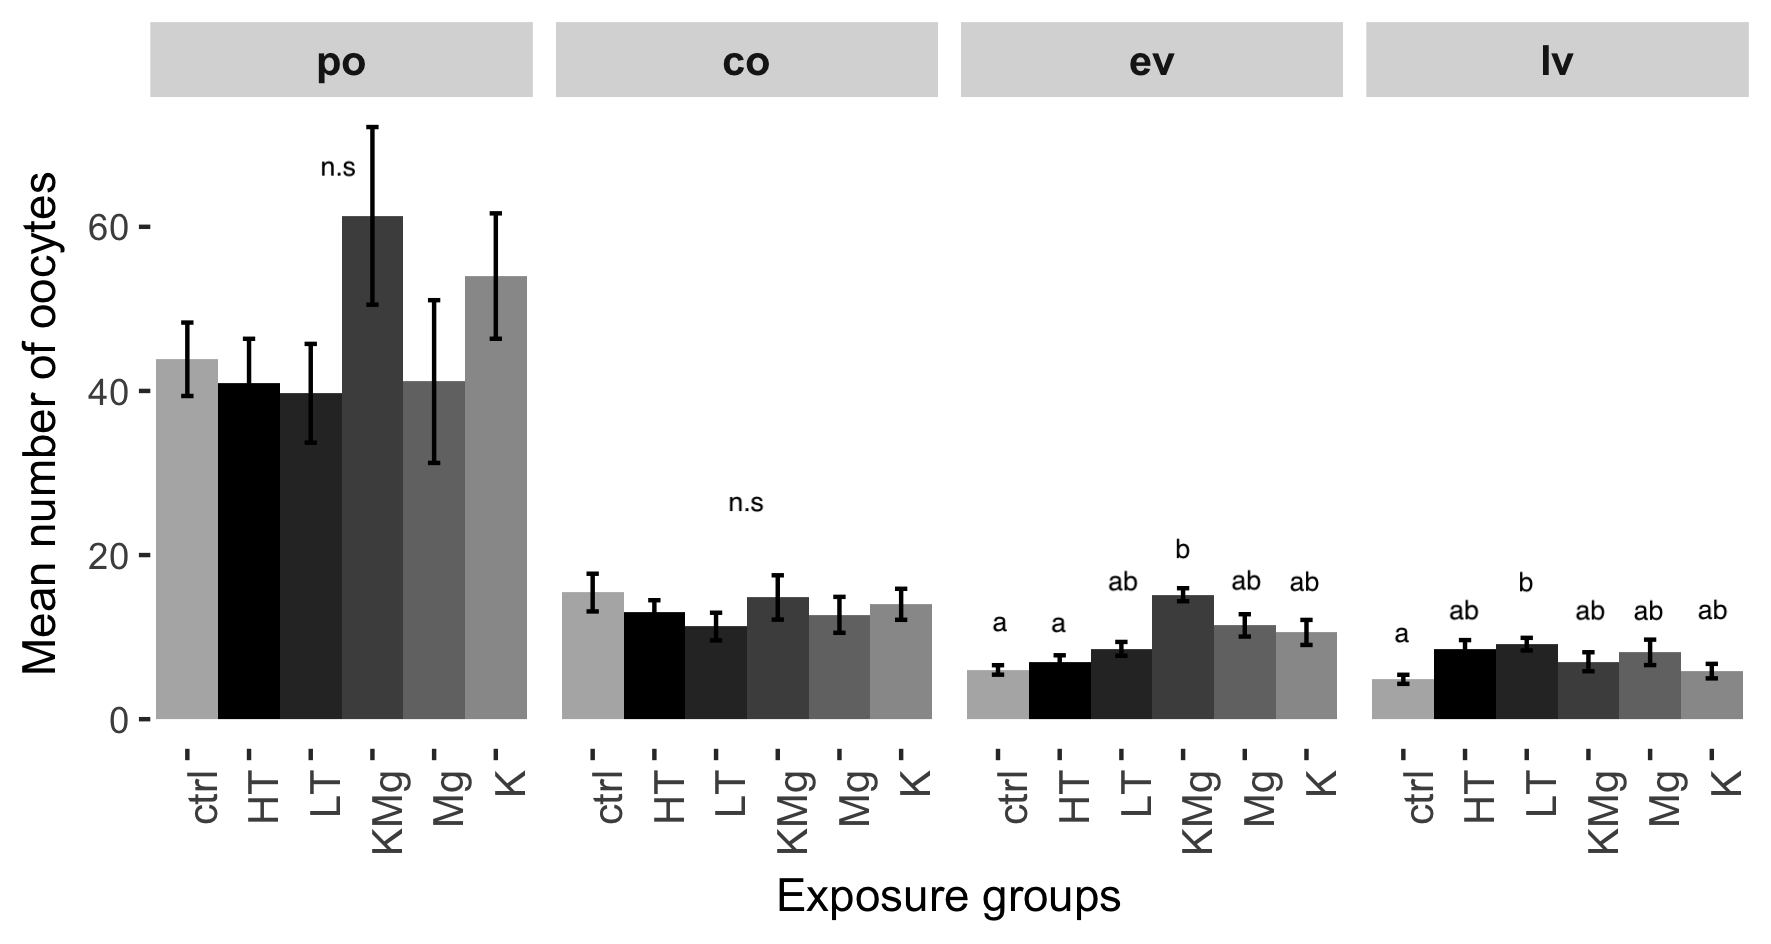
\includegraphics[scale=.117]{ggbarlot_ova_numb2.png}
\captionof{figure}{Mean number of developing oocytes $\pm$ SE for all groups in each stage. $^{a,b}$ indicate significant differences by one-way ANOVA and Tukey test (p < 0.05, \textit{N = 10}).}
 \label{fig:ovnumb}
\end{figure}
\FloatBarrier



\subsubsection{Testes}
In testes, the relative presence of spermatogenic cells in each stage varies from one treatment to another. However, in each group, spermatocysts (sc) were most abundant, spermatogonia (sg) least abundant, followed by spermatids (st). \\
A significant difference between groups in their proportion of spermatogenic cells could be found between ctrl and LT, KMg and Mg. LT, KMg and Mg had highly significantly more spermatogonia than ctrl. \\
Regarding spermatocysts, the difference between ctrl and LT was highly significant. Mg and K differed also significantly from ctrl. All were more abundant than ctrl. \\
For spermatids, LT, Mg and K exhibited significantly more cells than ctrl (Fig.:\ref{fig:tarea}).

\begin{figure}[H]
 \centering
 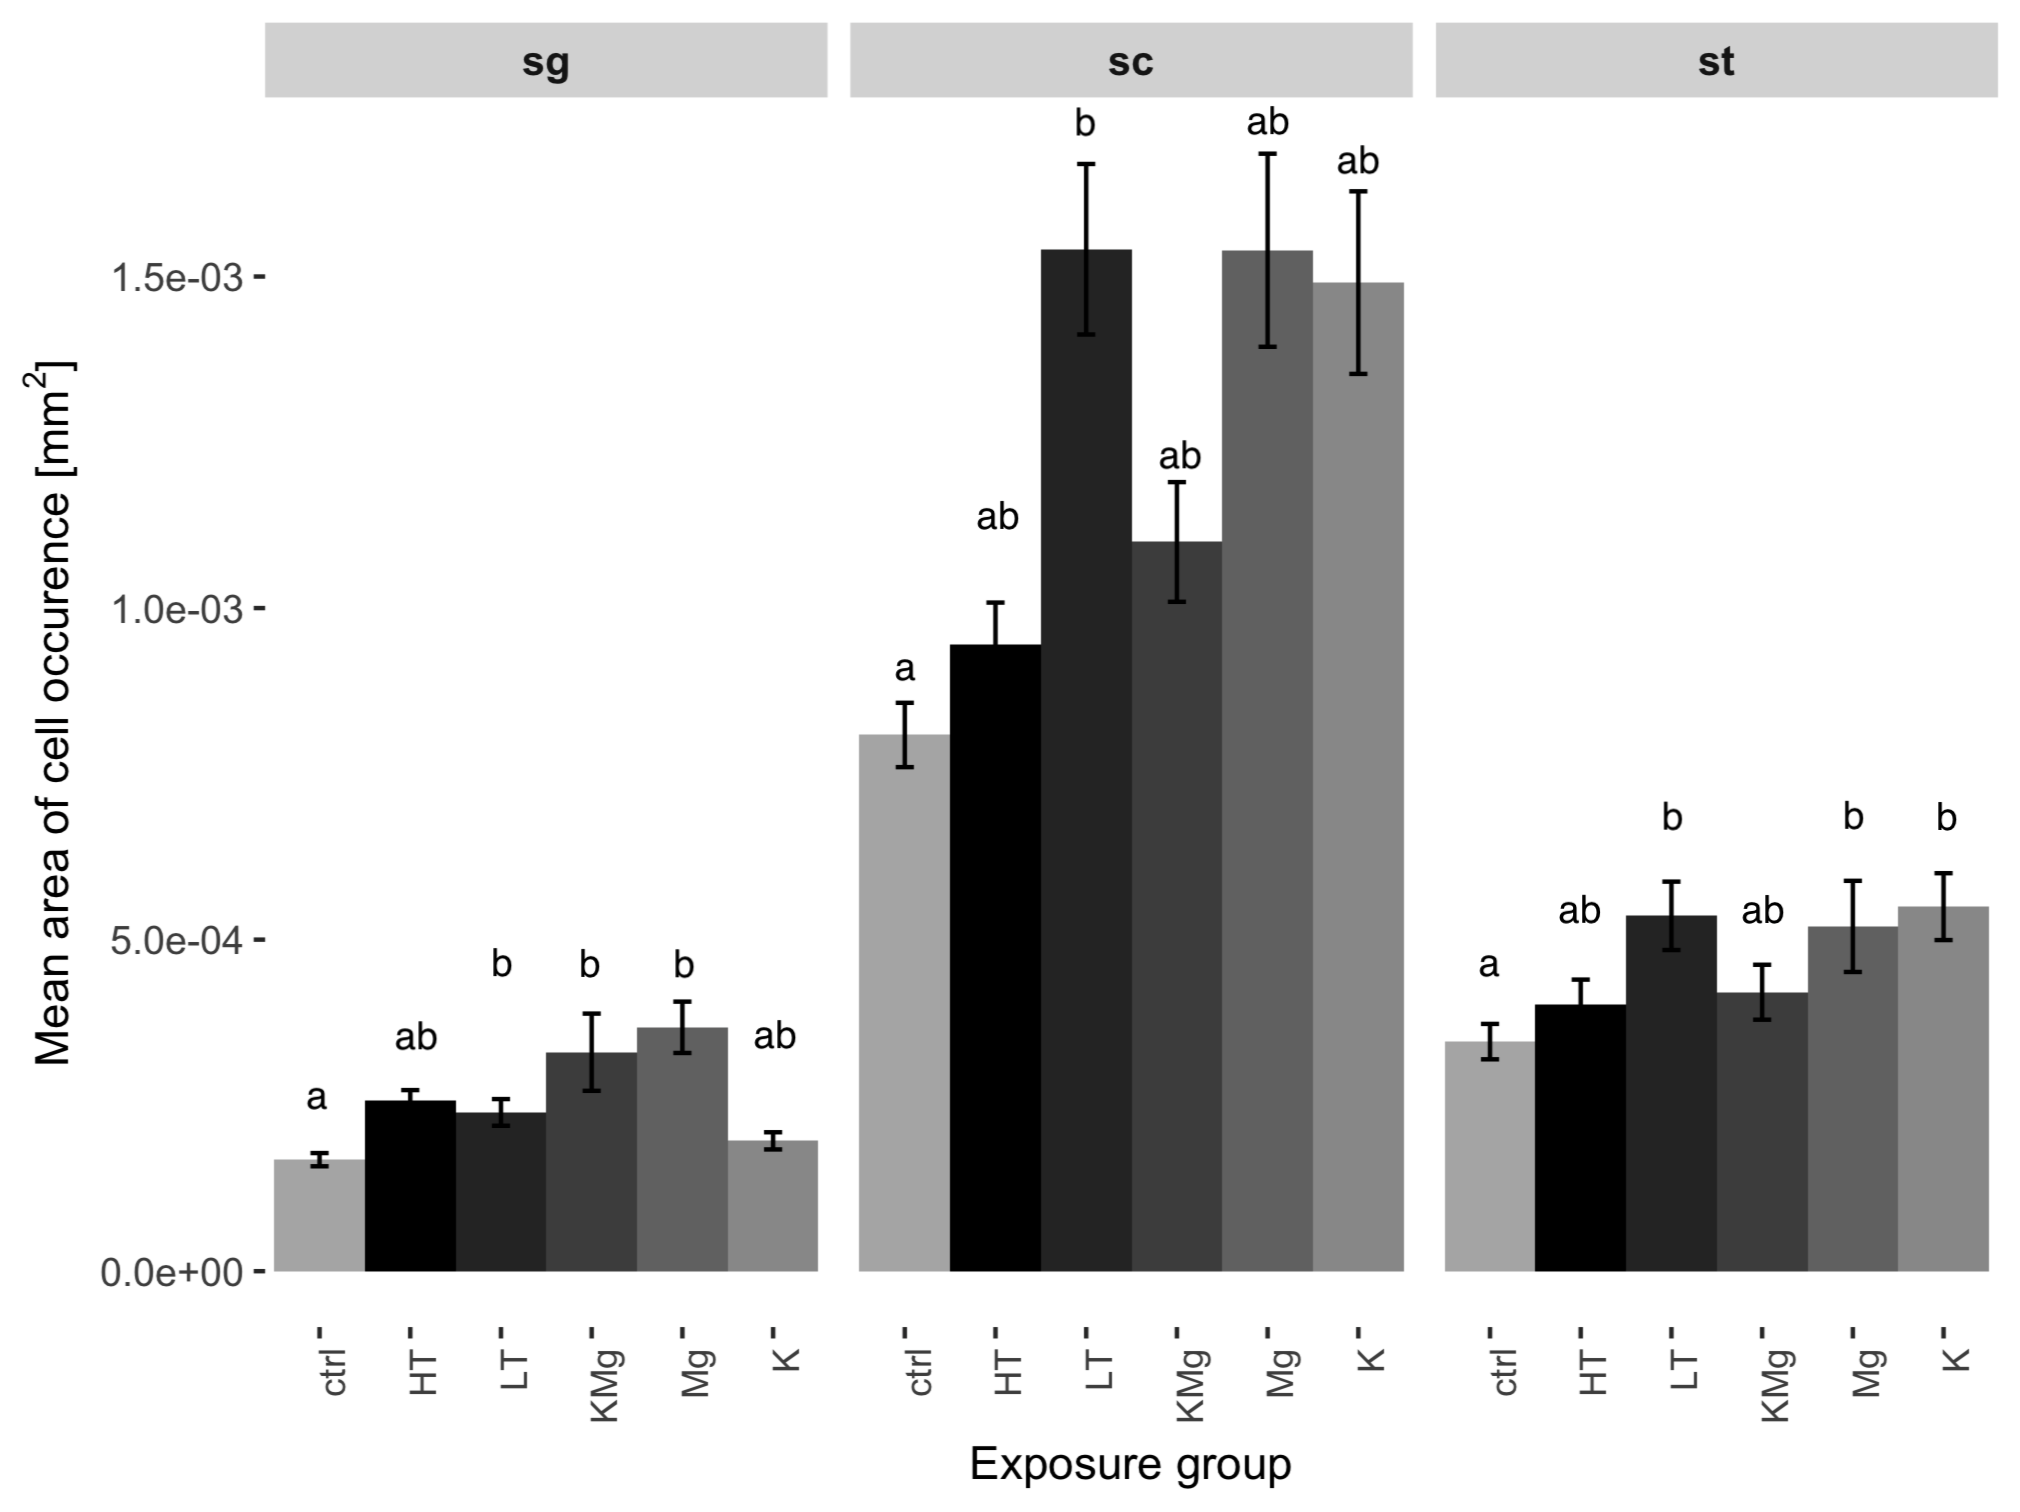
\includegraphics[scale=.1]{ggbarlot_testes133.png}
\captionof{figure}{Mean area of spermatogenic cells $\pm$ SE for all groups. $^{a,b}$ indicate significant differences by Kruskal-Wallis and Dunn's test (p < 0.05, \textit{N = 10}).}
 \label{fig:tarea}
\end{figure}
\FloatBarrier

\subsection{mRNA Expression}

\subsubsection{\textit{Fsh, lh, gh} \& \textit{pro}}
The relative expression levels of mRNAs are shown in Fig.: \ref{fig:horm}. The relative mRNA expression of \textit{fsh} did not indicate any significant differences for females. Expression levels for males on the other hand were highly significant as HT and LT were significantly higher than ctrl. Both were also significantly higher than KMg. \\
The relative mRNA expression of neither \textit{lh} nor \textit{gh} revealed any statistical significances for either sex.\\
The relative mRNA expression of \textit{pro} showed significant deviations for both sexes. In females, HT and LT were lower than ctrl, whereas \textit{pro} expression in Mg was significantly higher than HT and LT for male group members. 


\end{multicols}

\begin{figure}[H]
 \centering
 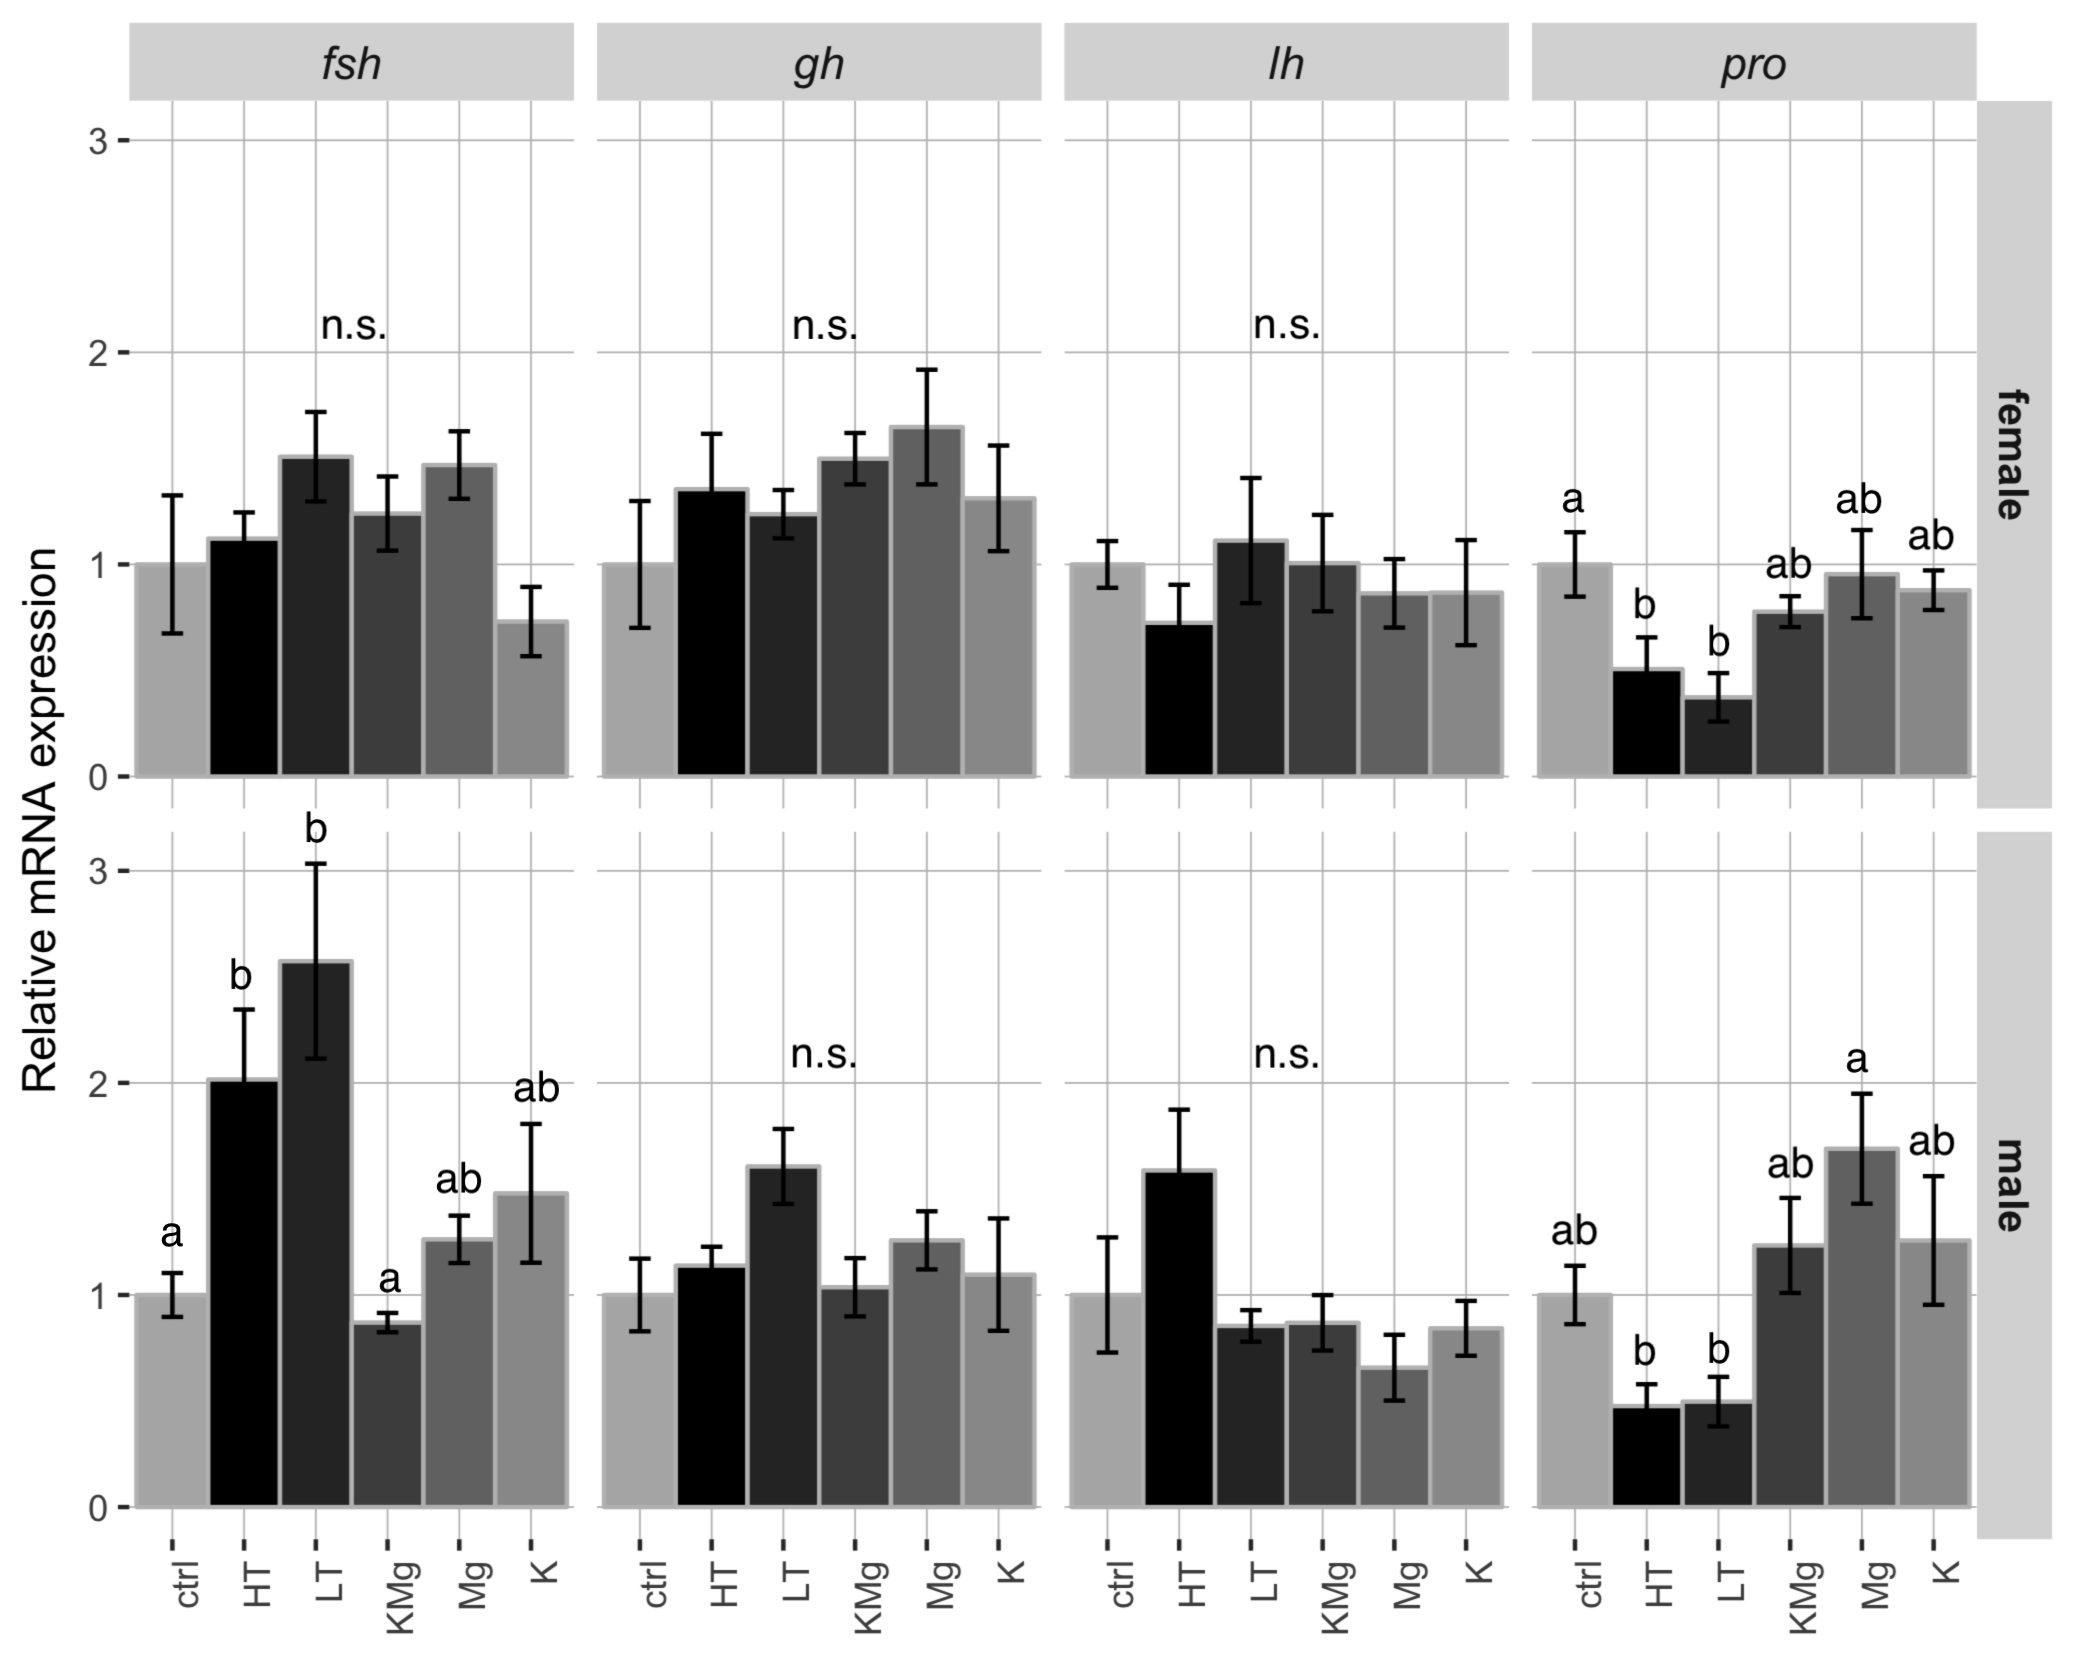
\includegraphics[scale=.2]{ggbarplot_hormall.png}
\captionof{figure}{Relative expression of \textit{fsh, gh, lh} and \textit{pro} $\pm$ SE for both sexes in all exposure groups. Expression in \% relative to ctrl which is displayed as 100\%. $^{a,b}$ indicate significant differences by Kruskal-Wallis and Dunn's test (p < 0.05). Sample size ranging from \textit{N = 5} to \textit{N = 7} per group.}
 \label{fig:horm}
\end{figure}
\FloatBarrier

\begin{multicols}{2}

\section{Discussion}
\lettrine[nindent=0em,lines=2]{T}{}
he results of this study revealed that after a six-week exposure all exposure groups elicited moderate and to a certain degree ion-specific effects on the different measured parameters. \\
\subsection*{Cortisol}
Cortisol is the most commonly used indicator for stress, due to its elevation in plasma in presence of a stressor and initiation of secondary (e.g. glucose, energy substrates) and tertiary stress (e.g. growth, reproduction) response factors \citep{Schreck2001}. Cortisol usually returns to basal levels shortly after the exposure to a stressor, but can also remain elevated for a prolonged time \citep{bonga1997}. \\
In both groups, HT and K, cortisol levels were significantly elevated after six weeks.  The persistently elevated cortisol levels suggest that individuals of both groups continuously experienced stress during the whole exposure time and point out the chronic effect of multiple ions in high concentrations, as well as the effect of a single ion, in this case K$^+$, in high concentration. However, although the effects were still measurable at the end of the long-term exposure, they were only minor in their expression and therefore indicate moderate stress.  \\ \\
Interestingly, this observed effect was diminished in association with Mg$^{2+}$ when regarding KMg. KMg cortisol levels were lower than the single cation enriched groups K and Mg. \\
Since no changes of the cortisol concentration were observed in the exposure groups LT, Mg and KMg, it can only be speculated whether an increased secretion of the stress hormone was induced but had already returned to basal levels.\\
Other studies have observed similar events where stressors of different nature induced an initial stress response, resulting in elevated cortisol levels that gradually decreased as the fishes were adapting \citep{jeney1997,kammerer2010}. Chronic stress manifests itself in strongly elevated cortisol levels over a prolonged period of time \citep{mazeaud1977,pickering1989}. Still, even under chronic stress conditions, cortisol concentrations eventually decreased to lower levels, initiated by different regulatory responses, leading to the so-called habituation \citep{barton1987,mommsen1999,jentoft2005}. \\
\cite{piato2011} exposed zebrafish to an unpredictable chronic stress and found that plasma cortisol levels were still elevated after 14 days. Even crowding can lead to elevated whole-body cortisol levels in \textit{D. rerio} lasting for several days \citep{ramsay2006}. \\  \\
Cortisol has been sufficiently described as the major factor reducing performance capacity, especially growth and reproduction, in fish under chronic stress \citep{bonga1997,pickering1981,Schreck2001}. \\ Long-term maintenance and adaptive changes in ion transport can vary under the presence of cortisol in both fresh- and seawater fish. This reflects the intimate relationship between energy metabolism and hydromineral control in fish \citep{bonga1997}. \\

\subsection*{Gill Histology}
Gills are multifunctional organs, which are responsible for gas exchange, intake and excretion of metabolites, acid-base-balance as well as osmoregulation \citep{Evans2008}. \\
Gills of all exposure groups showed significant structural changes compared to ctrl, however most alterations were of minimal or moderate impact. Each exposure group was characterised by hyperplasic filaments, meaning a proliferation of epithelial cells, followed by lifting/epithelial rupture and fusion. \\
Assessing the results, no general rule can be found to explain the magnitude of the response of the individuals to the corresponding exposure. HT and LT showed the most noticeable damage when regarding hyperplasia, but HT and K were highest in lifting. HT consistently remained the group with the most effects observed  for all alterations regarded. However, it is to say that the ion-concentration of all exposure groups had a negative effect on gill structure as all of them indicated alterations or damage. \\
It seems that an increased occurrence of one response leads to a further alteration. As an initial response, cells proliferate to increase the distance between tissue and water. An extensive dilatation of the lamellae caused neighbouring cells to move sideways, which led to deformations and fusions \citep{adriano2005,poleksic1999}. \\
All alterations indicated a structural change of the epithelium that covers the respiratory surface and forms the main barrier between the fish's blood and surrounding water. This results in an increased blood-to-water diffusion distance and reduction of interlamellar distance, also known as respiratory diffusion distance. Hyperplasia causes a direct thickening via proliferation of pavement, mucous and chloride cells \citep{Mcdonald1993}. Lifting, as a consequence of fluid infiltration has a similar effect: retarding toxicant uptake and disrupting tight junctions \cite{Wood2001}. \\
\cite{velasco2008} found out that high concentrations of NaCl had an irritant effect on gills of moneda (\textit{Metynnis orinocensis}) causing epithelia lifting, together with other lamellar changes such as oedema and severe epithelial separation. Fusion of secondary filaments also increases diffusion distance, thus affecting gas exchange \citep{Nowak1992}. \\ \\
All diagnosed findings can be seen as indicators of moderate effects as a result of the chronic ion stress induced on fish in this study. Furthermore, it is evident that all structural changes are protective responses and adaptation to the stressor. Given the fact, that gills are continually exposed to a fish's external environment, gills appear to be a frequent target for stress responses \citep{harper2009}. The most common alterations found in the literature are always related to surface reduction and interference with respiratory gas exchange. Perch exposed to high salinities responded with gill cell proliferation resulting in a reduced surface area and available lamellae for gas exchange \citep{nero2006}.  This also applies to this study, where excessive ions caused structural changes in gills decreasing surface area for active and passive ion exchanges. \\
Although changes in gill structure reduce salinity stress, the efficiency of gas exchange may be impacted and lead to long-term decrease in fish fitness \citep{shahriari2013}. The adaptations seem moderate, but little is known about how fish will be able to sustain vital function in the long-term.  \\

\subsection*{Gonad Histology}
\subsubsection*{Ovaries}
Four major classes of gonadal stages were categorised and analysed in terms of abundance and size. \\
A general observation for female gonads was that size and abundance of oocytes in the different groups showed considerable variation.  \\ Individuals, which were exposed to high single ion solutions (K and Mg) were bigger than the oocytes in multiple ion solutions (HT and KMg). Ctrl was in-between the two size categories and not significantly different to either.  \\
Oocytes of the other multiple ion solution LT were also bigger in size than HT and KMg.  LT was characterised by the occurrence of very late, or rather mature oocytes, which are bigger in size. Lv and mature/spawning oocytes were summarised into one group as the occurrence of very late ones was rare, thus the elevated size of lv  occytes for this group. In the other groups, there was very rarely a single mature, but rather lv or ev oocytes. \\
Abundance proportions between groups were never consistently the same along the stages of maturation. No notable effects were found in any stage, apart from KMg being more abundant in the vitellogenic stages ev and lv.
Size and abundance of oocytes in the vitellogenic stages indicate a negative relationship. \\ \\
The presence of late oocytes in LT are in accord with GSI outcomes, where LT depicted an elevated value compared to the control. \\ 
Variation in size structure can partially be explained by cortisol levels. Implanted cortisol has been shown to suppress ovarian growth in adult Tilapia experiencing chronic stress \citep{foo1993}  and guppies experiencing prolonged stress showed also reduced oocyte sizes \citep{dahlgren1979}. Cortisol was elevated in HT and in K, but oocyte size in HT was  reduced compared to K. \\ However, \cite{Heuts1947} found out, that the rate of development in many species of female freshwater fish was remarkably increased in media containing high ion concentrations. It is probable that different mechanisms to cope with stress, influencing ovarian growth, took place. \\

It is well known, that stress can impair an organism's ability to perform necessary life functions, including reproduction \citep{Schreck2001}. %(Christian, 1961; Schreck, 1981).
The timing in the life cycle, duration and severity of the stressor, as well as environmental factors play a crucial role and can lead to completely different responses depending on the species' reproductive strategy and its costs \citep{Schreck2001}. Reproduction can hereby be accelerated or inhibited \citep{schreck2010}. \\ 
As stressors affect energy allocation,  the most common trade-off in reproduction is between fecundity and life span \citep{Schreck2001}. Hence, the reproductive strategy has to favour either gamete quality or progeny fitness. Timing and duration of the stressor seem to have a considerable impact on egg size and number, as well as ovulation \citep{contreras1998,campbell1992,morehead2000}. 

%%%%%bisschen wiederholung kann man kürzen
\subsubsection*{Testes}
Three major stages of testicular maturation were analysed: spermatogonia (sg), spermatocytes (sc) and spermatids (st). Unlike ovaries, the testicular germ cells decrease in size but become more abundant with maturation before males release them into the water \citep{Leino}. \\
In the three stages of testes development only one clear pattern could be found: the relative presence of spermatogenic cells was consistently higher in LT and Mg compared to control. Sg in KMg and spermatids in K were also elevated. \\
GSI outcomes did not reveal any significant differences and can thus not confirm any associations with stress-related hormones. \\ \\ 
It is interesting that the abundance of mature cells was highest in LT for both females and males. The effect of stress hormones, such as cortisol, on reproductive strategies has been described numerous times for fishes \citep{pickering1981,bonga1997,Schreck2001}. The effect of stressors on reproduction can be hormetic/biphasic, where mild stress can have a positive effect on reproduction, while greater stress affects reproduction negatively.  The stress in LT seems to have been mild, in order to have the stimulating effect observed in this study. It is plausible, that the prolonged stress individuals in HT experienced, confirmed by cortisol levels, caused fish to delay reproductive processes in order conserve energy resources for other tasks. \\
Understanding shifts in reproduction strategies under adverse conditions are important for maintaining and managing natural populations, as well as stocks in aquaculture. 

\subsection*{mRNA Expression}
Stress induces a neuroendocrine cascade, where a complex relationship between stress-related hormones and reproductive hormones exists. The hormones discussed in this study are FSH, LH, GH and PRO. \\
The relative mRNA expression of \textit{fsh} for male fish are in accord with previous findings of this study. Levels of \textit{fsh} support the histological evaluation of male gonads. \textit{Fsh}  levels in males were also elevated in LT and a higher number of mature spermatocytes were found. As \textit{fsh} levels were also elevated in males in HT, similar results would have been assumed for histology of gonads and GSI outcomes of males. However,  outputs were not significant. \\
No effect was recorded for female \textit{fsh} levels. Furthermore, the addition of ions had no effect on \textit{lh} mRNA levels in any exposure group. \\ \\ 
\cite{pickering1987} found out, that rainbow trout experiencing long-term stress, with elevated cortisol even after four weeks, was accompanied by an elevation of the gonadotropins FSH and LH. However, other studies described that LH secretion, and to a lesser extent FSH, is decreased under long-term stress \citep{krulich1974,gray1978} or that gonadotropin levels remained unchanged \citep{billard1981}. \\ Clearly, there are other complex mechanism involved in the synthesis and secretion of these hormones, that can potentially interact, have inhibitory or stabilising effects. \\ \\ 
Interestingly, the energetically costly vitellogenin production in females, where both FSH and LH are involved, seems to be maintained in stressful conditions. There appears to be a buffering system that allows the maintenance of reproductive processes, probably at the expense of other functions \citep{schwindt2007}. Although the impairment of reproductive performance induced by stressors has been described for various stressors and for a great number of species \citep{krulich1974,gray1978,billard1981}, the effects described on gonadotropic hormones leave room for interpretation.  
\\ \\
Relative mRNA expression of prolactin, the hormone responsible for the development of freshwater chloride cell, was in both exposure groups with the high concentrated ion mixture, HT and LT, much lower compared to ctrl and other exposure groups. This can also confirm the ion-stress males and females in HT and LT were experiencing. Low levels of \textit{pro} serve as an indicator that fish in these two groups were already adapting on a hormonal level to high ion conditions and is correlated with other ion-stress induced symptoms observed. \cite{pottinger1992} also observed a reduction in plasma prolactin in relation to elevated cortisol in rainbow trout. \\ \\ 
PRO and GH are both from the same family of pituitary hormones and have similar functions that are greatly influenced by stressors.  However, GH did not reveal any significant effects. \\
GH has been mainly related to somatic growth and hydromineral control in teleost seawater fish, but has also growth-promoting capacities in sexual maturation and gonadal development \citep{pickering1989}. %(Pickering, 1990). 
Prolactin is a pivotal factor controlling the integumental permeability of fish in freshwater environments \citep{bonga1997}. However, both play a role in chloride-cell differentiation. \\
Two types of chloride-cells exist, the freshwater and the seawater type. They arise through epithelial differentiation during acclimation to different salinities. They differ from one another by their individual morphology and transport mechanisms \citep{Mccormick2001}. 
Development and differentiation of the freshwater chloride cell is regulated by prolactin, whereas growth hormone (GH) promotes the seawater acclimation. Salinity acclimation controlled by GH and prolactin involves regulation of cell proliferation, apoptosis, where cortisol is largely involved as well \citep{Sakamoto2006}. Considering the inhibitory effect of prolactin on the seawater-type chloride cell differentiation, prolactin expression levels as well as cortisol concentrations can be seen  as indictors for an  adaptation of HT and LT to elevated salinities. Consequently, chloride cell functioning was disturbed on a hormonal as well as on a structural level due to structural changes in gill morphology, leading to an impaired active ion uptake \citep{sardella2004}. \\ Surprisingly, \textit{gh} levels remained unchanged, which could be an indicator for a moderate effect/stress was not high enough and that an adaptation to elevated concentration was sufficient by suppressing prolactin secretion. Hence, a complete seawater acclimation was not necessary.  \\ \\ 
It is interesting, that the impacts of every cation combination on the measured parameters are not consistent. In some cases, K$^+$ and Mg$^{2+}$ induced an effect when their single ion concentrations were exceeding, but then in other cases they lead to an effect together (KMg). Sometimes ions together had a stabilising effect, but could also have an adverse effect. The change induced is therefore not always concentration-specific, but ion-specific.  However, testwaters with high concentration of all ions were consistently the ones inducing an effect. \\ 
Surprisingly, the impact of K$^+$, playing an important role in the cardiovascular system, were not as strong as expected, which suggests adaptation mechanisms of \textit{Danio rerio} to ion-stress. \\
Previous studies dealing with salinity focused on the effects of sodium-chloride, whereas results of this study give new insights into the effects of other ions. The results support our hypothesis that not only high concentrations, but also disproportions and the excess of single ions, compared to undisturbed conditions, can be harmful to a freshwater organism. \\ 
The energy costs of maintaining osmoregulatory homeostasis consume a high amount of a fish's energetic reserve. In the laboratory, the individuals were fed and exposed to a stable environment with consistent conditions. The ability to adjust physiologically and behaviourally to other physical stressor in a natural environment, i.e. forage, flight and weather, as well as the ability to reproduce and survive are reduced by the energetic expenses of chronic stress. \\
Although the effects in this study were rather moderate and show the robustness of adult \textit{Danio rerios}, further research on this subject by Wagler (Unpublished Data) determined a negative impact of high ion concentrations and single enriched media on fecundity, gamete quality and progeny fitness. 

\section*{Conclusion}
High concentrations of ions exert a feedback on adult zebrafish on almost all parameters analysed. Cortisol concentrations, histology of gills and gonads, as well as mRNA expression of \textit{fsh} and \textit{pro} were altered. \\
A physiological effect was exhibited on individuals from HT, LT and K by causing changes in cortisol concentrations and mRNA expressions. Cortisol levels of HT and K were still elevated after six weeks indicating that the fish had not fully acclimated to the ion-stress. \\ 
Structural changes of the gill of all exposure groups in order to increase the diffusing distance were observed.  \\ Reproductive parameters resulted in significant size variation for oocytes of LT and K and indicated higher \textit{fsh} expression levels for males in HT and LT. \\
Prolactin was lower in HT and LT, which is an indicator for a hormonal adaptation to seawater conditions.  \\
Altogether, the present investigation has demonstrated that chronic ion-stress clearly induces moderate effects on the reproductive performance of \textit{Danio rerio}. \\
The results of a laboratory study are only to a limited extent transferable to a real ecosystem. Ecological consequences, including effects on gamete quality and progeny fitness, as well as the potential effects of additional stressors affecting gill capacity and functional fitness, cannot be ruled out. \\
In this study, the fish were exposed for only six weeks, in a natural environment the exposure is of a much longer duration, where moderate effects could also become severe effects. If the organisms cannot adapt to these changes, or the energetic demand of adaptations is at the expense of other vital functions, the population's survival in the disturbed environment will be at risk. \\ 
For these reasons, current thresholds should be reconsidered/reevaluated, including thresholds for single ions and total ion concentration.  








\end{multicols}

\begin{multicols}{2}




%------------------------------------------------


\end{multicols}

%----------------------------------------------------------------------------------------
%	REFERENCE LIST
%----------------------------------------------------------------------------------------
\noindent\rule{\textwidth}{0.5pt}


\bibliography{bib2}










\end{document}






